%!TEX program = xelatex
\documentclass[aspectratio=43]{ctexbeamer}
% \usepackage{physics}  
                        %%% 宽高比说明 %%%%
%% ctexbeamer宏包支持各种宽高比,但本模板只适配了4:3(默认)和16:9的宽高比背景。
%% 添加选项aspectratio=169或aspectratio=43可以更改宽高比,默认是4:3
\usepackage[bluetheme]{ustcbeamer}
% !TeX root = ./main.tex

% 自适应16:9的宽高比设置
\makeatletter
\@ifclasswith{ctexbeamer}{aspectratio=169}{
		\def\backxscale{4/3}\def\backyscale{1}\def\ustcshift{30}
	}{
		\def\backxscale{1.068}\def\backyscale{1.068}\def\ustcshift{0}
	}
\makeatother

\newcommand{\maketitleframe}{
	%取消footline,sidebar
	\setbeamertemplate{footline}[footlineoff]
	%%设置本命令以后的背景如下
	\usebackgroundtemplate{%
			% !TeX root = ./main.tex
\begin{tikzpicture}[y=1pt, x=1pt, yscale=0.474*\backyscale, xscale=0.474*\backxscale, inner sep=0pt, outer sep=0pt]
    % \begin{scope}[cm={{1,0.0,0.0,-1,(0,0)}}]
      \path[fill=themecolor1,even odd rule] (720.4059,0.3515) -- (720.4059,71.1507) --
        (0.3436,71.1507) -- (0.3436,0.3515) -- cycle;
    
    
    
      \path[fill=themecolor2,even odd rule] (0.3436,76.0927) -- (720.4059,76.0927) --
        (720.4059,79.3043) -- (0.3436,79.3043) -- cycle;
    
    
    
      \path[left color=themecolor!80, right color=themecolor,even odd rule] (720.4059,392.4714) -- (0.3436,392.4714) --
        (0.3436,112.2780) -- (720.4059,112.2780) -- cycle;
    
    
    
          \path[even odd rule] (720.4059,392.4714) -- (0.3436,392.4714) --
            (0.3436,112.2780) -- (720.4059,112.2780) -- cycle;
    
    
    
      \path[fill=themecolor1,even odd rule] (0.3436,540.3980) -- (720.4059,540.3980) --
        (720.4059,433.5987) -- (0.3436,433.5987) -- cycle;
    
    
    
      \path[fill=themecolor,even odd rule] (84.0129,392.4714) -- (64.1007,392.4714) ..
        controls (139.6636,296.8146) and (237.7485,213.1007) .. (369.3679,152.9909) ..
        controls (258.0055,213.1787) and (160.4523,292.5573) .. (84.0129,392.4714) --
        cycle(0.3436,210.9419) -- (0.3436,112.2780) -- (205.1827,112.2780) .. controls
        (135.2103,142.0132) and (67.0535,175.1304) .. (0.3436,210.9419) --
        cycle(0.3436,318.0849) -- (0.3436,261.2429) .. controls (87.4868,197.7318) and
        (173.6552,147.4217) .. (257.6874,112.2780) -- (329.6364,112.2780) .. controls
        (208.4627,165.2559) and (97.0387,225.2988) .. (0.3436,318.0849) --
        cycle(23.7974,392.4714) -- (0.3436,392.4714) -- (0.3436,375.5798) .. controls
        (103.8628,248.3597) and (243.0859,163.2623) .. (385.7678,112.2780) --
        (411.7601,112.2780) .. controls (266.1313,174.0682) and (125.2848,246.4444) ..
        (23.7974,392.4714);
    
    
    
      \path[fill=themecolor2,even odd rule] (0.3436,428.6568) -- (720.4059,428.6568) --
        (720.4059,425.4452) -- (0.3436,425.4452) -- cycle;

      \node at(185-\ustcshift,488){\textcolor{themecolor}{
\includegraphics[scale=1]{./theme/ustc_logo_side.pdf}}};
    % \end{scope}
\end{tikzpicture}
	}%
	%封面页
	\begin{frame}%
		\maketitle%
	\end{frame}%
	%设置本命令以后的背景如下
	\usebackgroundtemplate{%
			% !TeX root = ./main.tex
\begin{tikzpicture}[y=1pt, x=1pt, yscale=0.474*\backyscale, xscale=0.474*\backxscale, inner sep=0pt, outer sep=0pt]
% \begin{scope}[cm={{1,0.0,0.0,-1,(0,0)}}]
    \path[left color=themecolor!80,right color=themecolor,even odd rule] (720.4059,540.3980) -- (0.3436,540.3980) --
      (0.3436,478.8258) -- (720.4059,478.8258) -- cycle;



        \path[even odd rule] (720.4059,540.3980) -- (0.3436,540.3980) --
          (0.3436,478.8258) -- (720.4059,478.8258) -- cycle;



    \path[fill=themecolor,even odd rule] (84.0129,540.3980) -- (64.1007,540.3980) ..
      controls (139.6636,519.3777) and (237.7485,500.9814) .. (369.3679,487.7725) ..
      controls (258.0055,500.9987) and (160.4523,518.4420) .. (84.0129,540.3980) --
      cycle(0.3436,500.5071) -- (0.3436,478.8258) -- (205.1827,478.8258) .. controls
      (135.2103,485.3599) and (67.0535,492.6376) .. (0.3436,500.5071) --
      cycle(0.3436,524.0517) -- (0.3436,511.5606) .. controls (87.4868,497.6042) and
      (173.6552,486.5485) .. (257.6874,478.8258) -- (329.6364,478.8258) .. controls
      (208.4627,490.4677) and (97.0387,503.6621) .. (0.3436,524.0517) --
      cycle(23.7974,540.3980) -- (0.3436,540.3980) -- (0.3436,536.6860) .. controls
      (103.8628,508.7296) and (243.0859,490.0294) .. (385.7678,478.8258) --
      (411.7601,478.8258) .. controls (266.1313,492.4040) and (125.2848,508.3087) ..
      (23.7974,540.3980);

  \path[fill=themecolor2,even odd rule] (720.4059,475.6141) -- (0.3436,475.6141) --
    (0.3436,478.8258) -- (720.4059,478.8258) -- cycle;



  \path[fill=themecolor,even odd rule] (0.3436,0.3515) -- (720.4059,0.3515) --
    (720.4059,28.5100) -- (0.3436,28.5100) -- cycle;



  \path[fill=themecolor2,even odd rule] (720.4059,28.5100) -- (0.3436,28.5100) --
    (0.3436,31.7217) -- (720.4059,31.7217) -- cycle;

  \node at(580+\ustcshift,509){\textcolor{white}{
\includegraphics[scale=0.8]{./theme/ustc_logo_side.pdf}}};



% \end{scope}

\end{tikzpicture}
	}%
}%
%
                        %%% ustcbeamer说明 %%%%
%% 宏包使用了TikZ代码形式的背景文件(在子文件夹theme中),默认选项"bluetheme",是科大校徽的蓝色;此外ustcbeamer还内置了红色和黑色主题"redtheme","blacktheme"。

                        %%% 自定义你的主题颜色 %%%
%% 一旦使用了下述命令就会覆盖ustcbeamer的内置颜色选项,你可以设置自己喜欢的RGB色值:
% \definecolor{themecolor}{RGB}{0,150,0} % 这是绿色主题
% \definecolor{themecolor}{RGB}{0,150,150} % 青色主题,也蛮好看的

%% 注意小写rgb和大写RGB表示的色值相差255倍,即RGB{255,255,255}=rgb{1,1,1};
% \definecolor{themecolor}{rgb}{0,0.5,0.3} % 深绿色主题

%% 建议自定义的主题颜色选择偏深色
%%%%%%%%%%%%%%%%%%%%%%%%%%%%%%%%%%%%%%%%%%%%%%%%%%%%%%%%%%%%%%%%%%%%%%


\title[布料仿真]{
    布料仿真:加速的十年
}
\author[]{}
\institute[]{

}
\date{\today}
\begin{document}
%\section<⟨mode specification⟩>[⟨short section name⟩]{⟨section name⟩}
%小于等于六个标题为恰当的标题

%--------------------
%标题页
%--------------------
\maketitleframe
%--------------------
%目录页
%--------------------
%beamer 101
\begin{frame}%
	\frametitle{Contents}%
	\tableofcontents[hideallsubsections]%仅显示节
	%\tableofcontents%显示所节和子节
\end{frame}%
%--------------------
%节目录页
%--------------------
\AtBeginSection[]{
\setbeamertemplate{footline}[footlineoff]%取消页脚
  \begin{frame}%
    \frametitle{Contents}
	%\tableofcontents[currentsection,subsectionstyle=show/hide/hide]%高亮当前节,不显示子节
    \tableofcontents[currentsection,subsectionstyle=show/show/hide]%show,shaded,hide
  \end{frame}
\setbeamertemplate{footline}[footlineon]%添加页脚
}
%--------------------
%子节目录页
%--------------------
\AtBeginSubsection[]{
\setbeamertemplate{footline}[footlineoff]%取消页脚
  \begin{frame}%
    \frametitle{Contents}
	%\tableofcontents[currentsection,subsectionstyle=show/hide/hide]%高亮当前节,不显示子节
    \tableofcontents[currentsection,subsectionstyle=show/shaded/hide]%show,shaded,hide
  \end{frame}
\setbeamertemplate{footline}[footlineon]%添加页脚
}

\section{布料仿真的常见方法}
\subsection{弹簧质点系统}
\begin{frame}
  \frametitle{弹簧质点系统}
        \; \;布料在发生形变时,需要考虑系统内部的相对影响,通过弹簧可以模拟布料形变时产生的弹性势能。首先将布料用网格表示,给网格的顶点一定的质量,通过弹簧将网格的顶点相连构成弹簧质点系统。
        \begin{center}
            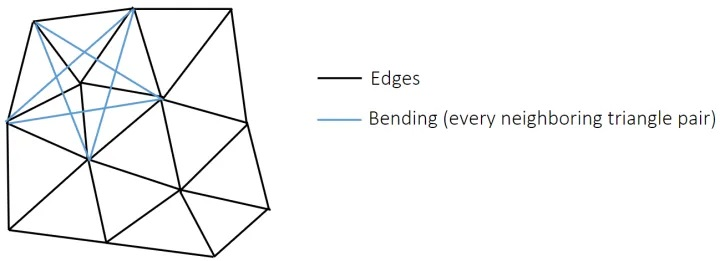
\includegraphics[width=1.0\linewidth]{./fig/弹簧质点模型.jpg}
        \end{center}
\end{frame}

\begin{frame}
  \frametitle{弹簧质点系统}
        在不考虑非保守力的作用下,系统中质点的位置可以唯一地确定系统的状态。利用牛顿第二定律:
        \begin{equation}
			x''=M^{-1}(\frac{\partial E}{\partial x})
        \end{equation}

		在弹簧质点系统中,根据胡克定律(Hooke's law):
        \begin{equation}
		\begin{split}
			&F_{spring}=-k_s\Delta x \\
			&F_{s_i}=k_s(1-\frac{L}{\left \| x_i-x_j \right \| })(x_i-x_j)
		\end{split}
        \end{equation}
​		除此之外还可以加入重力、空气阻力、弹簧阻尼等其它作用力。
\end{frame}

\begin{frame}
  \frametitle{弹簧质点系统}
​		在模拟系统随时间的演化时,求解(2)式得到:
        \begin{equation}
            x = \iint M^{-1}(\frac{\partial E}{\partial x}+F)dtdt=\iint adtdt
        \end{equation}

		在实际的模拟中,时间是离散的,因此需要做数值积分。直接的方法是显式欧拉方法(explicit Euler method):
        \begin{equation}
		\begin{split}
			v(i+1) = v(i) + a(i)\Delta t \\
			x(i+1) = x(i) + v(i)\Delta t
		\end{split}
        \end{equation}
		此时下一时刻的速度和位移完全由上一时刻决定,导致当$\Delta t$较大时计算结果不稳定。
\end{frame}

\begin{frame}
  \frametitle{弹簧质点系统}
		另一种方法是隐式欧拉方法(implicit Euler method):
        \begin{equation}
		\begin{split}
			v(i+1) = v(i) + a(i+1)\Delta t \\
			x(i+1) = x(i) + v(i+1)\Delta t
		\end{split}
        \end{equation}
		由于加速度也是位置的函数,此时需要解方程得出下一时刻的速度,它的误差比显式欧拉方法小一些。

		在隐式欧拉方法中,将速度方程代入位置方程可以得到:
		\begin{equation}
		\begin{split}
			x(i+1)= x(i) + v(i)\Delta t + M^{-1}f(i+1)(\Delta t)^2
		\end{split}
		\end{equation}
        \begin{equation}
			\frac{M}{(\Delta t)^2}(x(i+1)-x(i)-v(i)\Delta t) - f(i+1)=0
        \end{equation}
\end{frame}

\begin{frame}
  \frametitle{弹簧质点系统}
		在不考虑非保守力时,可以构造一个优化问题,使$x(i+1)$为这个优化问题的解,从而利用求解优化问题的方法求解数值积分:
		\begin{equation}
		\begin{split}
			&F(x)=\frac{1}{2(\Delta t)^2}(x-\bar x)^TM(x-\bar x)+E(x)\\
			&\bar x=x(i)+v(i)\Delta t\\
			&x(i+1) = \mathop{argmin}\limits_xF(x)
		\end{split}
		\end{equation}

		考虑系统可能发生的碰撞,最终需要求解的问题为:
		\begin{equation}
		\begin{split}
			&x(i+1) = \mathop{argmin}\limits_xF(x)\\
			&s.t. \quad x(i+1) \in  \Omega
		\end{split}
		\end{equation}
\end{frame}

\begin{frame}
  \frametitle{弹簧质点系统}
		当系统与连续体发生碰撞时:
        \begin{equation}
			s.t. \quad tx(i+1) +(1-t)x(i) \in  \Omega \quad t\in[0,1]
        \end{equation}

		为了求解这个优化问题,可以使用牛顿法,利用下面的公式进行迭代直到收敛:
        \begin{equation}
			x^{k+1} = x^{k}-(\nabla ^2F(x))^{-1}\nabla F(x)
        \end{equation}
		初始的$x^0=x(i)$,最终收敛的$x^{k}=x(i+1)$
\end{frame}

\subsection{弹性模型}
\begin{frame}
  \frametitle{弹性模型}
		\; \;将布料抽象成三角形的网格,处理当三角形网络发生形变时所带来的的能量变化:

		\begin{itemize}
			\item[$\bullet$] 当三角形的边长改变时需要能量
			\item[$\bullet$] 当两个相邻三角形的夹角发生变化时需要能量
			\item[$\bullet$] 当三角形需要变形或剪切时需要能量
		\end{itemize}

		\; \;在能量发生变化时需要相应的力做功,因此可以通过系统的状态推出系统内部各质点之间的相互作用力。
\end{frame}

\begin{frame}
  \frametitle{弹性模型}
		也可以在相邻三角形上加上弹簧以抵抗弯曲。

        \begin{center}
            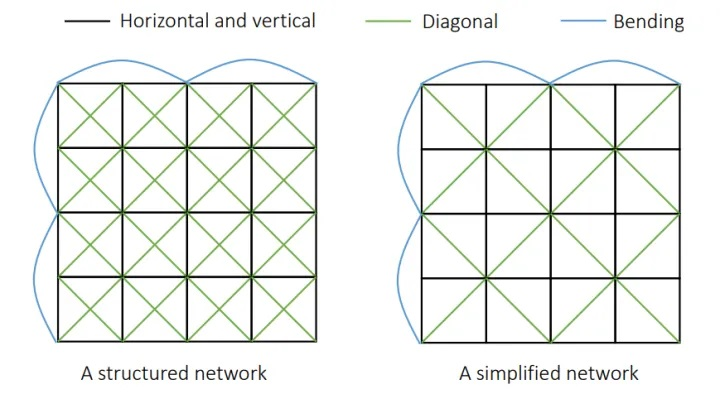
\includegraphics[width=1.0\linewidth]{./fig/三种弹簧.jpg}
        \end{center}
\end{frame}

\subsection{基于位置的动力学方法}
\begin{frame}
  \frametitle{基于位置的动力学方法}
        \begin{center}
            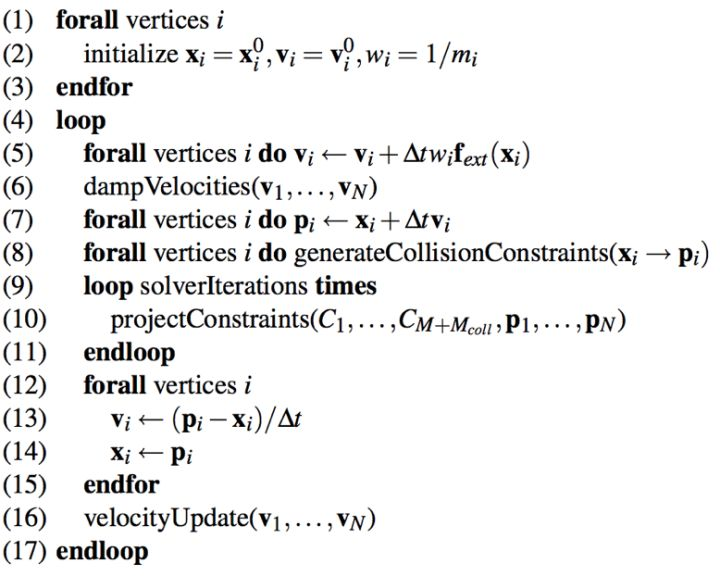
\includegraphics[width=0.8\linewidth]{./fig/PBD算法.jpg}
        \end{center}
\end{frame}

\begin{frame}
  \frametitle{基于位置的动力学方法}
		假设有一个n维约束:
		\begin{equation}
		\begin{split}
			&\pmb{p} = [\pmb{p_1},…,\pmb{p_n}]\\
			&C(\pmb{p}) = 0
		\end{split}
		\end{equation}

		现在需要找到偏移量$\Delta \pmb{p}$,使得投影前的$\pmb{p}$在偏移后满足约束:
        \begin{equation}
			C(\pmb{p}+\Delta \pmb{p})=0
        \end{equation}

		对约束函数在$\pmb{p}$处进行展开:
        \begin{equation}
			C(\pmb{p}+\Delta \pmb{p}) = C(\pmb{p}) + \nabla_pC(\pmb{p}) \cdot \Delta \pmb{p} +o(\Delta \pmb{p}) =0
        \end{equation}
\end{frame}

\begin{frame}
  \frametitle{基于位置的动力学方法}
		将$\Delta \pmb{p}$限定在$\nabla_pC(\pmb{p})$的方向上可以保持动量、角动量守恒:
        \begin{equation}
			\Delta \pmb{p} = \lambda \nabla_pC(\pmb{p})
        \end{equation}

		联立可得:
        \begin{equation}
			\Delta \pmb{p} = -\frac{C(\pmb{p})}{\left | \nabla_pC(\pmb{p}) \right | ^2}\nabla_pC(\pmb{p})
        \end{equation}

		对于单个质点来说:
        \begin{equation}
		\Delta \pmb{p_i} = -\frac{C(\pmb{p})}{\sum_{j} \left | \nabla_{p_j}C(\pmb{p}) \right | ^2}\nabla_{p_i}C(\pmb{p})
        \end{equation}
\end{frame}

\begin{frame}
  \frametitle{基于位置的动力学方法}
		考虑到质点的$\Delta \pmb{p_i}$应与质量的倒数$\omega_i=\frac{1}{m_i}$成反比
        \begin{equation}
\Delta \pmb{p_i} = -\frac{C(\pmb{p})}{\sum_{j} \omega_j\left | \nabla_{p_j}C(\pmb{p}) \right | ^2}\omega_i\nabla_{p_i}C(\pmb{p})
        \end{equation}

		对于布料,两个质点之间的距离约束可以表述为:
        \begin{equation}
			C(\pmb{p_1},\pmb{p_2})=\left | \pmb{p_1}-\pmb{p_2} \right |-L
        \end{equation}

		梯度为:
		\begin{equation}
		\begin{split}
			&\nabla_{p_1}C(\pmb{p_1},\pmb{p_2})=\frac{\pmb{p_1}-\pmb{p_2}}{\left | \pmb{p_1}-\pmb{p_2} \right |}\\
			&\frac{C(\pmb{p})}{\sum_{j} \omega_j\left | \nabla_{p_j}C(\pmb{p}) \right | ^2} = \frac{\left | \pmb{p_1}-\pmb{p_2} \right |-L}{2}
		\end{split}
		\end{equation}
\end{frame}

\begin{frame}
  \frametitle{基于位置的动力学方法}
		约束投影后的偏移为:
        \begin{equation}
		\Delta \pmb{p_1} =-\frac{1}{2}(\left | \pmb{p_1}-\pmb{p_2} \right |-L)\frac{\pmb{p_1}-\pmb{p_2}}{\left | \pmb{p_1}-\pmb{p_2} \right |}
        \end{equation}

		以下为两种迭代的方法,其中Gauss-Seidel遍历全部约束,难以进行并行。
        \begin{center}
            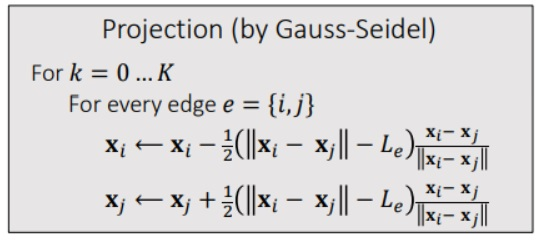
\includegraphics[width=0.7\linewidth]{./fig/PBD(Gauss-Seidel).jpg}
        \end{center}
\end{frame}

\begin{frame}
  \frametitle{基于位置的动力学方法}
		Jacobi方法在遍历全部约束后统一更新。
        \begin{center}
            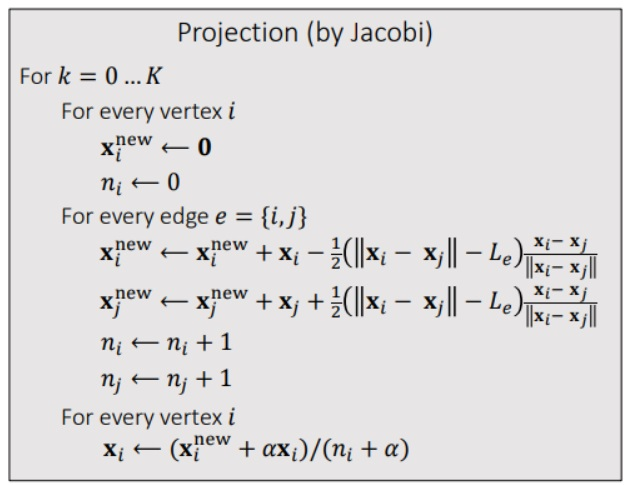
\includegraphics[width=0.7\linewidth]{./fig/PBD(Jacobi).jpg}
        \end{center}
\end{frame}

\begin{frame}
  \frametitle{基于位置的动力学方法}
		\; \;对于两个约束Ci和Cj,Gauss-Seidel和Jacobi方法的直观对比如下
        \begin{center}
            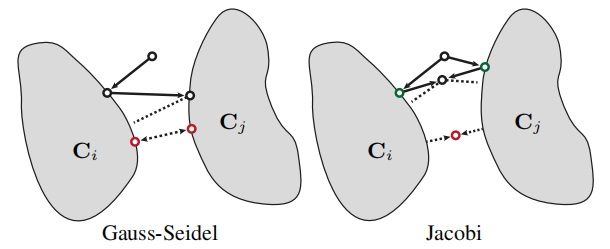
\includegraphics[width=0.7\linewidth]{./fig/Gauss-Seidel-Jacobi.jpg}
        \end{center}
		\; \;PBD方法系统的刚度取决于迭代的次数,迭代次数越多时约束越强,系统的刚度也就越大,然而很难得到一个物体的力学性质和迭代次数的关系。与隐式欧拉法相比,PBD优化的目标是$E(x)$,这使得它忽略了惯性项$\frac{1}{2(\Delta t)^2}(x-\bar x)^TM(x-\bar x)$,同时它不是基于物理推导出来的,不符合物理规律。
\end{frame}

\section{常见的线性方程组求解方法}
\begin{frame}
  \frametitle{常见的线性方程组求解方法}
		直接法:LU 分解、LDLT 分解、Cholesky 分解
		\begin{itemize}
			\item[$\bullet$] 代价高,得到精确解
			\item[$\bullet$] 对矩阵限制少
			\item[$\bullet$] 适合 CPU 计算
		\end{itemize}

		迭代法:Jacobi
		\begin{itemize}
			\item[$\bullet$] 如果需要得到精确解的话代价大,但是可以根据容差控制
			\item[$\bullet$] 要让方法收敛的话,对矩阵 有比较严格的限制(例如正定)
			\item[$\bullet$] 可使用GPU并行
			\item[$\bullet$] 实现比较容易
			\item[$\bullet$] 有很多加速算法
		\end{itemize}
\end{frame}

\section{论文调研}
\subsection{基于块式梯度下降的隐式欧拉法}
\begin{frame}
  \frametitle{基于块式梯度下降的隐式欧拉法}
	(2013)Fast Simulation of Mass-Spring Systems\\[10pt]

		\; \;在隐式欧拉法中,最后需要求解一个优化问题,除了用牛顿法外,还可以用块式梯度下降的方法,与牛顿法相比它们收敛到同一结果,虽然在渐进收敛速度上比牛顿法慢,但在不追求精度的情况下,并不需要迭代到最终收敛,这个方法在单步迭代的速率上快于牛顿法,因此在初始的几步迭代中能够快速减小误差同时取得与牛顿法相似的结果。
\end{frame}

\begin{frame}
  \frametitle{基于块式梯度下降的隐式欧拉法}
        \begin{center}
            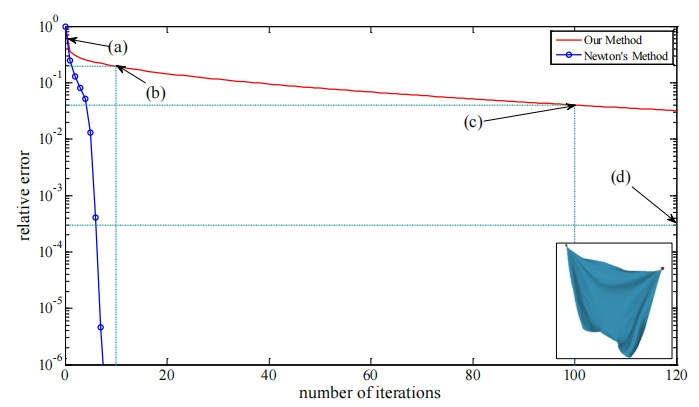
\includegraphics[width=1.0\linewidth]{./fig/块式梯度下降与牛顿法.jpg}
        \end{center}
\end{frame}

\begin{frame}
  \frametitle{基于块式梯度下降的隐式欧拉法}
		\; \;对于弹簧的弹性势能:
       \begin{equation}
			\frac{1}{2}\sum_{i=1}^{s}k_{i}||\mathbf{p}_{i_{1}}-\mathbf{p}_{i_{2}}-\mathbf{d}_{i}||^{2}={\frac{1}{2}}\mathbf{x}^{\mathsf{T}}\mathbf{L}\mathbf{x}-\mathbf{x}^{\mathsf{T}}\mathbf{J}\mathbf{d}
		\end{equation}

		\; \;得到最终的优化问题:
       \begin{equation}
			\operatorname*{min}_{{{\bf x}\in{\bf R}^{3},{\bf d}\in U}}\;\;\frac{1}{2}{\bf x}^{\bf T}({\bf M}+\Delta t^2{\bf L}){\bf x}-\Delta t^2{\bf x}^{\bf T}{\bf J}{\bf d}+{\bf x}^{\bf T}{\bf b}
		\end{equation}

		\; \;从x的初始猜测(显式欧拉法的结果)开始,交替优化x和d,其中优化x时是一个凸二次最小化问题,${\bf M}+\Delta t^2{\bf L}$是一个在迭代中不变的正定矩阵,可以对其预先计算其Cholesky分解从而加快速度。

		\; \;这个方法与PBD相比,正确地考虑了惯性项$\frac{1}{2}{\bf x}^{\bf T}{\bf M}{\bf x}$的存在,同时弹簧的刚性也被包括在${\bf L}$和${\bf J}$中。
\end{frame}

\subsection{投影动力学(Projective Dynamics)}
\begin{frame}
  \frametitle{投影动力学(Projective Dynamics)}
	(2014)Projective Dynamics Fusing Constraint Projections for Fast Simulation\\[10pt]

		PD是一个对物理系统进行隐式欧拉积分的新方法,可以将约束转换为势能部分,将势能表示为两部分的和:

       \begin{equation}
			W({\bf q},{\bf p})=d({\bf q},{\bf p})+\delta_{\mathrm{E}}({\bf p})
		\end{equation}

		其中$\delta_{\mathrm{E}}({\bf p})$形式化了p应该位于约束流形上的要求,$d({\bf q},{\bf p})$用于衡量p和q之间的距离,对p最小化方程(30)等价于寻找q在约束流形上的投影,因此对于材料模型$\Psi$产生的弹性势$W({\bf{q}})\,\,=\,\,\Psi({\bf{E}}({\bf{q}}))=\operatorname*{min}_{\mathbf{P}}W(\mathbf{Q},\mathbf{p})$
\end{frame}

\begin{frame}
  \frametitle{投影动力学(Projective Dynamics)}
        \begin{center}
            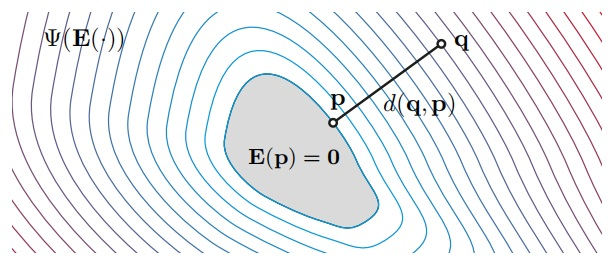
\includegraphics[width=1.0\linewidth]{./fig/材料弹性势.jpg}
        \end{center}
		\; \;将势能代入隐式欧拉积分中,采取交替优化的方法,先基于当前的q求出p,再根据新的p更新q,反复迭代直到收敛。

		\; \;$d({\bf q},{\bf p})$可取为简单的线性函数,这样在p固定时优化q变为线性优化问题,从而可以快速计算,而非线性的部分在优化p的过程中进行,这与[1]的思想类似。
\end{frame}

\subsection{SOR在PBD算法上的应用}
\begin{frame}
  \frametitle{SOR在PBD算法上的应用}
	(2014)Unified Particle Physics for Real-Time Applications\\[10pt]

		在优化视角下,PBD算法等价于:
		\begin{equation}
		\begin{split}
			&\mathrm{minimize}\quad \frac{1}{2}\Delta x^{T}M\Delta x\\ 
			&\mathrm{subject\;to}\quad C_{i}(x+ \Delta x)=0,\quad i=1,\cdot\cdot,n			
		\end{split}
		\end{equation}
		寻找满足约束条件的动能的最小变化,与高斯最小拘束原理一致。

		为了解决Gauss-Seidel方法不能并行的问题,可以先并行地处理每个约束,在迭代结束时将它们的均值作为最终的结果,并引入一个全局参数控制SOR的速率:
       \begin{equation}
			\Delta\tilde{\bf x}_{i}=\frac{\omega}{n_{i}}\Delta{\bf x}_{i}
		\end{equation}

\end{frame}

\subsection{PD算法的Chebyshev加速}
\begin{frame}
  \frametitle{PD算法的Chebyshev加速}
	(2015)A Chebyshev Semi-Iterative Approach for Accelerating Projective and Position-based Dynamics\\[10pt]

		注意到PD算法的收敛性与线性系统高度相似,因此可以使用Chebyshev加速来加速PD算法的收敛,其中谱半径从其收敛速度中估计得到。
\end{frame}

\begin{frame}
  \frametitle{PD算法的Chebyshev加速}
		Chebyshev加速方法易于实现,且与GPU加速兼容,其算法流程如下
        \begin{center}
            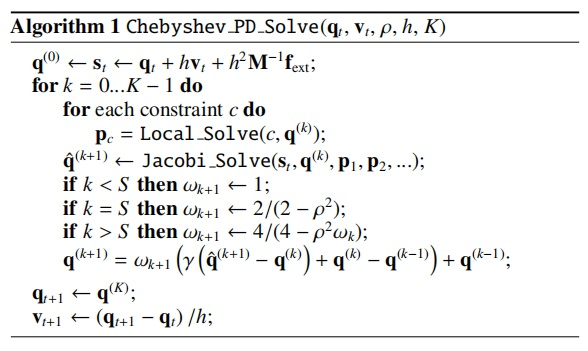
\includegraphics[width=0.7\linewidth]{./fig/chebyshev.jpg}
        \end{center}
\end{frame}

\begin{frame}
  \frametitle{PD算法的Chebyshev加速}
		\; \;Chebyshev加速方法还需要谱半径$\rho$,设估计的谱半径为$\hat \rho$,当$\hat \rho = 0$时,这个方法退化为不加速的迭代法,当$0 < \hat \rho < \rho$时,随着$\hat \rho$的增大收敛速度提升,一旦$\rho < \hat \rho$,会产生震荡,因此需要准确估计谱半径大小。

		\; \;由于PD有类似于线性系统的收敛性,把$\rho$作为每个问题中的常数,通过预模拟以估计$\rho$。首先将$\rho$初始化为$\left|\left|\mathbf{e}^{(K)}\right|\right|_{2}/\left|\left|\mathbf{e}^{(K-1)}\right|\right|_{2}$,其中误差被定义为$\mathrm{e}^{(k)}=\nabla\epsilon(\mathbf{q}^{(k)})$,然后多次调整$\rho$并进行仿真,找到收敛速度最大的$\rho$。

\end{frame}

\begin{frame}
  \frametitle{PD算法的Chebyshev加速}
        \begin{center}
            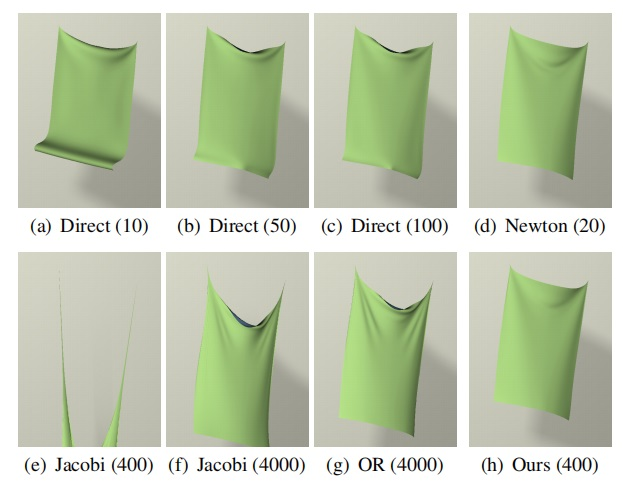
\includegraphics[width=0.8\linewidth]{./fig/Chebyshev加速对比.jpg}
        \end{center}
\end{frame}

\subsection{XPBD}
\begin{frame}
  \frametitle{XPBD}
	(2016)XPBD Position-Based Simulation of Compliant Constrained Dynamics\\[10pt]

		\; \;PBD算法中时间步长和迭代次数决定了物体的刚性,在复杂的系统中,由于参数之间的耦合,难以单独改变一个物体的刚性。在这篇文章中,提出了拓展的PBD算法(XPBD),显式引入弹性势能,从而通过弹性势能来确定物体刚性。
\end{frame}

\begin{frame}
  \frametitle{XPBD}
		\; \;弹性势能场为:
       \begin{equation}
			U({\bf x})={\frac{1}{2}}{\bf C}({\bf x})^{T}\alpha^{-1}{\bf C}({\bf x})
		\end{equation}

		\; \;最终得到新的迭代方程:
       \begin{equation}
		\begin{split}
			\Delta{\bf x}={\bf M}^{-1}\nabla\mathrm{C}({\bf x}_{i})^{T}\Delta\lambda \\
			\Delta\lambda_{j}=\frac{-C_{j}({\bf x}_{i})-\bar{\alpha}_{j}\lambda_{i j}}{\nabla C_{j}\mathrm{M}^{-1}\nabla(C_{j}^{T}+\tilde{\alpha}_{j}}
		\end{split}
		\end{equation}
\end{frame}



\begin{frame}
  \frametitle{XPBD}
        \begin{center}
            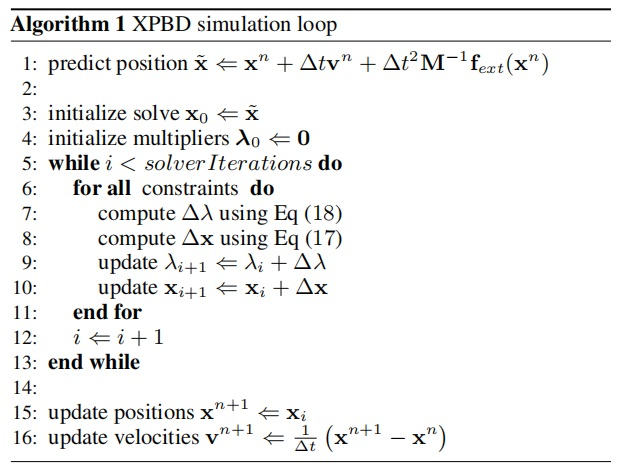
\includegraphics[width=0.8\linewidth]{./fig/XPBD算法.jpg}
        \end{center}
\end{frame}

\subsection{多重网络}
\begin{frame}
  \frametitle{多重网络}
	(2018)Parallel Multigrid for Nonlinear Cloth Simulation\\[10pt]

		\; \;多重网格法是迭代方法的一种,可用于求解线性方程组。

		\; \;一般的迭代法在求解线性方程组$A\phi=b$基于固定的步长进行迭代得到$\phi ^n$,对残差$r=b-A\phi^{n}$进行傅里叶变换可以把它们分解成一系列不同频率的残差,在迭代中对于频率较高的残差消除的较快,对频率低的残差消除的慢。可以通过增大步长来等价地提高频率,从而消除低频误差,但步长大时精度较低,因此可以在不同的步长上交替进行,在保持精度的同时加快误差消除,这被称为多重网格法。
\end{frame}

\begin{frame}
  \frametitle{多重网络}
        \begin{center}
            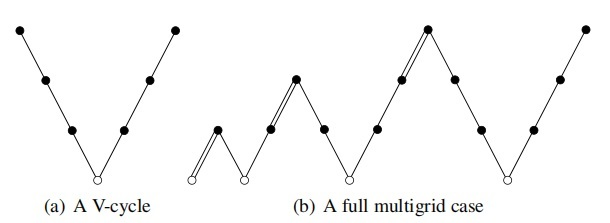
\includegraphics[width=0.7\linewidth]{./fig/multigrid.jpg}
        \end{center}
		
		图中黑色圆点代表平滑,白色圆点代表精确求解器,\textbackslash 和/代表限制和插值,//代表高阶插值,限制和插值用于粗细网格结果之间的映射。
\end{frame}

\subsection{基于深度学习的服装CG生成}
\begin{frame}
  \frametitle{基于深度学习的服装CG生成}
	(2019)Learning an Intrinsic Garment Space for Interactive Authoring of Garment Animation\\[10pt]

		\; \;衣物的生成通常通过物理模拟来实现,通过设置不同的物理参数,可以生成不同材质、形状的衣服。但是,为一个CG来生成衣服需要对于每一帧动作指定对应的物理参数,而这个参数和动作,前后帧都是有关系的。

		\; \;为了减少参数设置的工作量,需要在关键帧之间自动生成对应的衣服,但关键帧之间的运动可能非常复杂,衣服的生成无法直接通过插值得到,因此通过深度学习的方式找到衣服所对应的潜在空间,从而将衣物应用到不同的动作上。
\end{frame}

\begin{frame}
  \frametitle{基于深度学习的服装CG生成}
        \begin{center}
            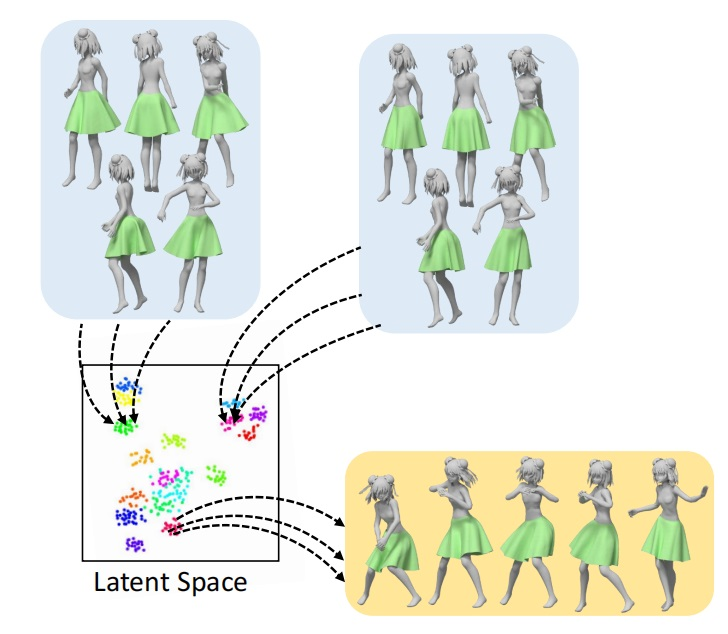
\includegraphics[width=0.7\linewidth]{./fig/潜在空间.jpg}
        \end{center}
\end{frame}

\begin{frame}
  \frametitle{基于深度学习的服装CG生成}
​		\; \;通过自动编码器进行服装网格与形状描述符之间的编码与解码,运动标签与运动描述符之间的编码与解码,将服装描述符和运动描述符降维到潜在空间中,其中运动描述符作为形状描述符到潜在空间的编码器的子网权重,再通过新的运动描述符重新变换回服装网络。

        \begin{center}
            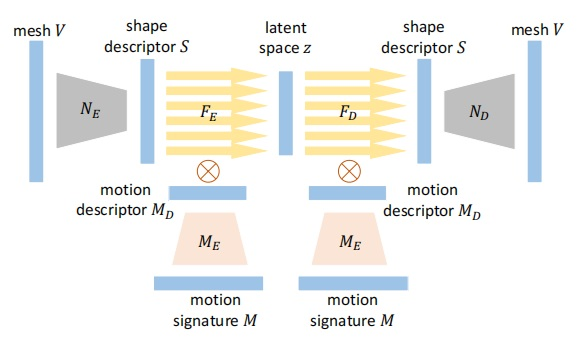
\includegraphics[width=0.6\linewidth]{./fig/auto-encode.jpg}
        \end{center}
\end{frame}

\begin{frame}
  \frametitle{基于深度学习的服装CG生成}
        \begin{center}
            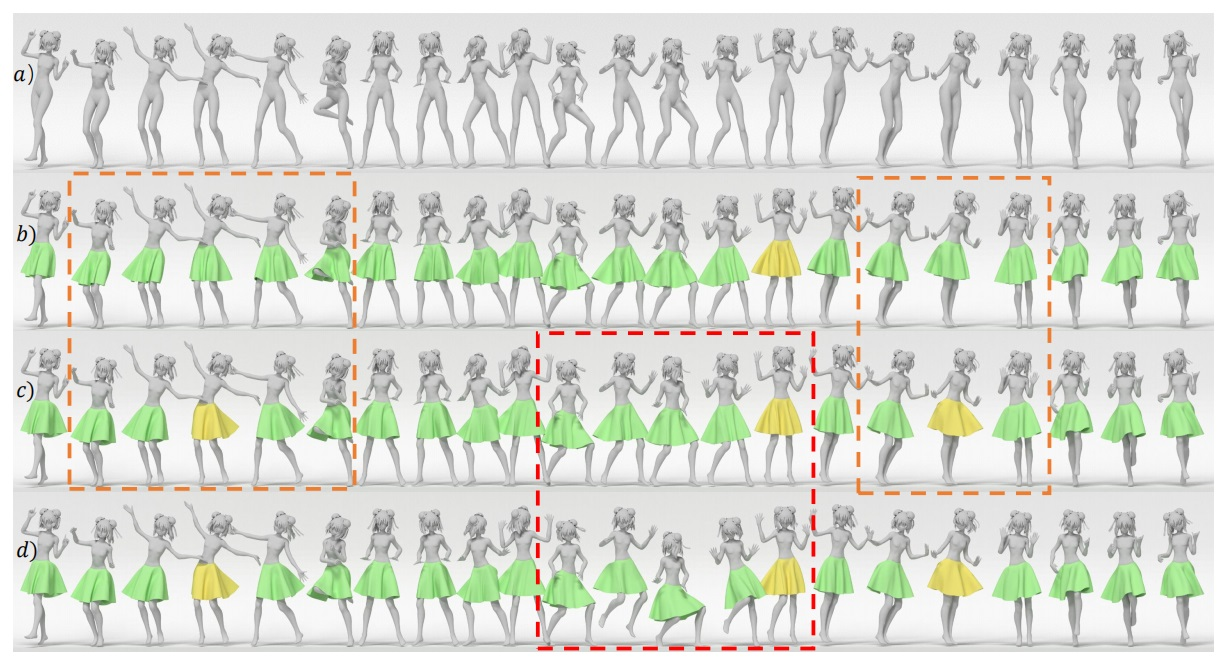
\includegraphics[width=1.0\linewidth]{./fig/animation.jpg}
        \end{center}
\end{frame}

\subsection{Incremental Potential Contact}
\begin{frame}
  \frametitle{Incremental Potential Contact}
	(2020)Incremental Potential Contact Intersection- and Inversion-free, Large-Deformation Dynamics\\[10pt]

		为了处理仿真中产生的碰撞,可以将碰撞视为一种约束,从而转化为优化问题。一般的隐式欧拉优化目标为:
       \begin{equation}
		\begin{split}
			&E(x,x^{t},v^{t})=\frac{1}{2}(x-\hat{x})^{T}{\cal M}(x-\hat{x})-h^{2}x^{T}f_{d}+h^{2}\Psi(x)\\
			&\hat{x}=x^{t}+h v^{t}+h^{2}M^{-1}f_{e}\\
			&x^{t+1}=\arg\operatorname*{min}_{x}E(x,x^{t},v^{t}),\quad x^{\tau}\in\cal{A}
		\end{split}
		\end{equation}
		其中$\cal{A}$为不发生碰撞的空间区域
\end{frame}

\begin{frame}
  \frametitle{Incremental Potential Contact}
		IPC方法将约束条件融合到目标函数中:
       \begin{equation}
			\arg\operatorname*{min}_{x}E(x)=\frac12\|x-x^{*}\|_{M}^{2}+h^{2}\Psi(x)+\kappa\sum_{k\in C}b(d_{k}(x))
		\end{equation}
\end{frame}

\begin{frame}
  \frametitle{Incremental Potential Contact}
        \begin{center}
            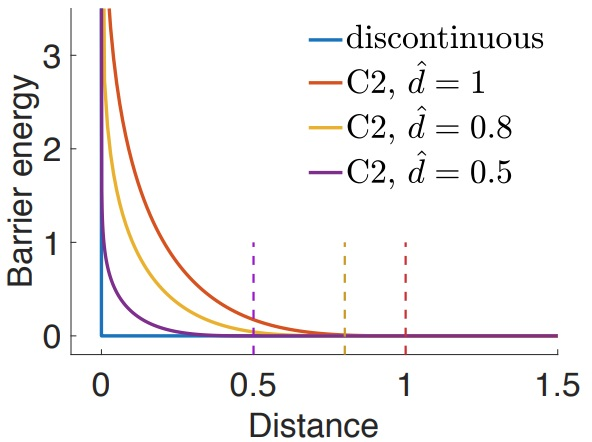
\includegraphics[width=0.7\linewidth]{./fig/障碍势能.jpg}
        \end{center}
\end{frame}

\subsection{高分辨率布料褶皱模拟}
\begin{frame}
  \frametitle{高分辨率布料褶皱模拟}
	(2021)GPU-Based Simulation of Cloth Wrinkles at Submillimeter Levels\\[10pt]

		传统的布料仿真使用非结构化的三角形网络,但这会带来巨大的内存开销和计算成本,在较高分辨率下三角形网络的灵活性不再重要,可以使用规则网络,提高内存访问的效率。
		
\end{frame}

\begin{frame}
  \frametitle{高分辨率布料褶皱模拟}
		在高分辨率下模拟布料褶皱的流程如下
        \begin{center}
            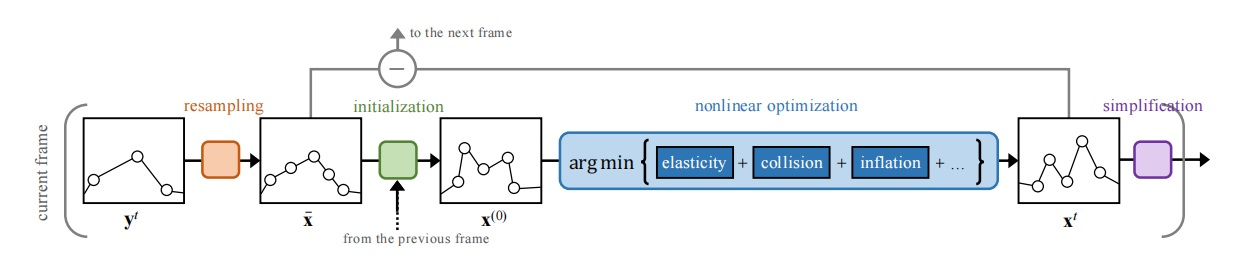
\includegraphics[width=1.0\linewidth]{./fig/褶皱模拟流程.jpg}
        \end{center}
		输入一个非结构化的网络,通过一个规则网络重新采样,然后运行一个初始化步骤来估计网格上的褶皱,通过非线性优化来生成褶皱的细节,最终将褶皱简化以便下一步处理。
\end{frame}

\begin{frame}
  \frametitle{高分辨率布料褶皱模拟}
		\; \;为了提升收敛速度,使用GPU来并行处理,可以在不重叠的GPU线程块中使用共享内存,这是由网格分区所自然创建的。但在每次迭代中每个块都需要将其部分从全局内存加载到共享内存中,如果块能够覆盖全部顶点,那就可以一次性加载共享内存,在顶点较多时,如果我们只为同一个不重叠的GPU块中的线程运行内部迭代,就可以重用只加载一次的共享内存数据。
\end{frame}

\end{document}
